\documentclass[12pt,a4paper]{article}
\usepackage[T2A]{fontenc}
\usepackage[utf8]{inputenc}
\usepackage[russian]{babel}
\usepackage{amsmath}
\usepackage{amssymb}
\usepackage{graphicx}
\usepackage{floatrow}
\usepackage{booktabs}
\usepackage{wrapfig}
\usepackage{lipsum}
\usepackage{subcaption}
\usepackage{fancyhdr}

\newcommand{\figref}[1]{(См. рис. \ref{#1})}
\newcommand{\secref}[1]{(См. раздел. \ref{#1})}

\newcommand{\e}[1]{\text{$\cdot10^{#1}$}}

\pagestyle{fancy}
\fancyhead{}
\fancyhead[L]{Работа 3.2.1}
\fancyhead[R]{}
\fancyfoot[C]{\thepage}

\author{\normalsize Выполнил: Голубович Тимур, группа Б01-108 \\
	\normalsize 05.11.2022}
\date{}

\usepackage{float}
\restylefloat{table}
\title{
	\large Отчет о выполнении лабораторной работы 3.2.1 \\
	\Large Сдвиг фаз в цепи переменного тока \\ 
	
}

\begin{document}
	\maketitle
	
\section*{Цель работы}
Изучить влияние активного сопротивления, индуктивности и ёмкости на сдвиг фаз между током и напряжением в цепи переменного тока.


\section*{Оборудование и приборы} 
Генератор звуковой частоты (ЗГ); 
двухканальный осциллограф (ЭО); 
магазин ёмкостей; 
магазин сопротивлений; 
катушка индуктивности; 
резисторы; 
универсальный измеритель (LCR-метр).

	
\section*{Теоретическое введение}

		Измерять сдвиг фаз в цепях переменного тока можно с помощью осицллографа. Пусть нужно измерить сдвиг фаз между двумя напряжениями $U_1$ и $U_2$. Можно предложить два способа измерения. В первом способе подадим эти напряжения на соответсвующие входы осциллографа. Смещения луча определяются 
		$$ x = x_0\cos\omega t \qquad y = y_0\cos\left(\omega t +\psi\right), $$
		где $\psi$ -- сдвиг фаз между напряжениями $U_1$ и $U_2$, а $x_0$ и $y_0$ -- амплитуды напряжений, умноженные на коэффициенты усиления соответсвующих каналов осцилографа.
		Исключим время:
		$$ \left(\frac{x}{x_0}\right)^2 + \left(\frac{y}{y_0}\right)^2+\frac{2xy}{x_0y_0}\cos\psi = \sin^2\psi.$$
		
        \begin{figure}[h!]
        	\centering
        	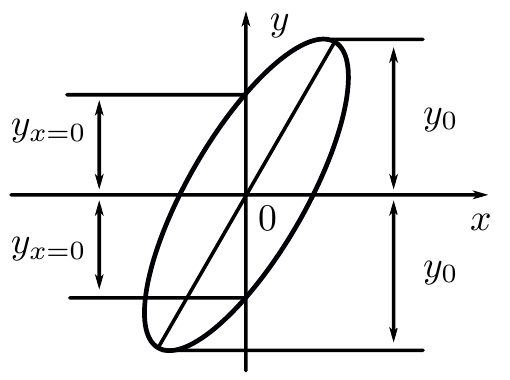
\includegraphics[width=6cm]{res/el.png}
        	\caption{Эллипс на экране осциллографа}
        	\label{fig:f}
        \end{figure}	
	
		Это выражение определяет эллипс на экране осциллографа. Для расчёта сдвига фаз можно измерить отрезки $2y_{x=0}$ и $2y_0$ и, подставляя эти значения в уравнение эллипса, найдем
		
		\begin{equation}
		    \label{eq:1}
		    \psi = \pm\arcsin\left(\frac{y_{x=0}}{y_0}\right).
		\end{equation}
		
		Для правильного измерения отрезка $2y_{x=0}$ важно, чтобы центр эллипса лежал на оси $y$.
		
		Второй способ заключается в непосредственном измерении сдвига фаз между сигналами на экране двухканального осциллографа. Для измерения разности фаз удобно:
		
		1) подобрать частоту горизонтальной развёртки, при которой на экране укладывается чуть больше половины периоды синусоиды;
		
		2) отцентрировать горизонтальную ось;
		
		3) измерить расстояние $x_0$ (см. рис. \ref{fig:s1}) между нулевыми значениями одного из сигналов, что соответсвует разности фаз $\pi$;
		
		4) измерить расстояние $x$ между нулевыми значениями двух синусоид и пересчитать в сдвиг по фазе: 
		
		\begin{equation}
		    \label{eq:2}
		    \psi = \pi x / x_0.
		\end{equation}
		
		На практике применяются фазовращатели. Используя метод комплексных амплитуд, найдём зависимость сдвига фаз между входным и выходным напряжением в зависимости соотношения между импедансами сопротивления $R$ и ёмкости $C$. Для этого выразим выходное напряжение через параметры контура и частоту внешнего источника.
		
		Пусть комплексная амплитуда входного напряжения $\mathbf{U_\text{вх}}$. Тогда напряжение между точками 1 и 3 (рис. \ref{fig:s2}) в силу равенства сопротивлений:
		$$\mathbf{U_{13}} = \frac{\mathbf{U_\text{вх}}}{2}.$$
		Пусть фаза входного напряжения равна нулю, тогда $\mathbf{U_\text{вх}}$ будет действительной величиной. Примем напряжение в точке 1 равным нулю, тогда:
		$$\mathbf{U_{03}} = \frac{\mathbf{U_\text{вх}}}{2}$$
		Рассчитаем амплитуду в точке 4. Импеданс последовательно соединенных емкости и сопротивления равен 
		$$Z = R - \frac{i}{\omega C}.$$
		Для комплексной амплитуды тока $\mathbf{I_\text{вх}}$, проходящего через R и C, имеем
		$$\mathbf{I_\text{вх}} = \frac{\mathbf{U_\text{вх}}}{Z}=\cfrac{\mathbf{U_\text{вх}}}{R-\cfrac{i}{\omega C}},$$
		а для комплексной амплитуды напряжения в точке 4 ---
		$$ \mathbf{U_{04}} = \mathbf{I_\text{вх}}R = \mathbf{U_\text{вх}}\cfrac{R}{R-\cfrac{i}{\omega C}}$$
		Тогда выходное напряжение:
		$$ \mathbf{U_{\text{вых}}} = \mathbf{U_{04}}-\mathbf{U_{03}} = \mathbf{U_{04}}-\frac{\mathbf{U_\text{вх}}}{2}.$$
		Окончательно получаем:
		
		\begin{equation}
		    \mathbf{U_\text{вых}} = \frac{\mathbf{U_\text{вх}}}{2}\cfrac{R+\cfrac{i}{\omega C}}{R - \cfrac{i}{\omega C}}.
		\end{equation}
		
		Величина выходного напряжения не меняется, посколько модули комплексных величин одинаковы. Сдвиг фаз равен:
		
		\begin{equation}
		    \psi = \arg \frac{\mathbf{U_\text{вых}}}{\mathbf{U_\text{вх}}} = 2\arctan\left(\frac{1}{\omega RC}\right).
		\end{equation}
		
		Он может меняться от $\psi=\pi$ при $R\rightarrow 0$ до $\psi=0$ $\frac{\pi}{2}$ при $R\rightarrow \infty$.

	\section*{Экспериментальная установка}

    Схема установки для исследования сдвига фаз между током и напряжением в цепи переменного тока представлена на рис. \ref{fig:s1}. Эталонная катушка $L$, магазин ёмкостей $C$ и магазин сопротивлений $R$ соединены последовательно и через дополнительное сопротивление $r$ подключены к источнику синусоидального напряжения -- звуковому генератору (ЗГ).
    
    \begin{figure}[h!]
    	\centering
    	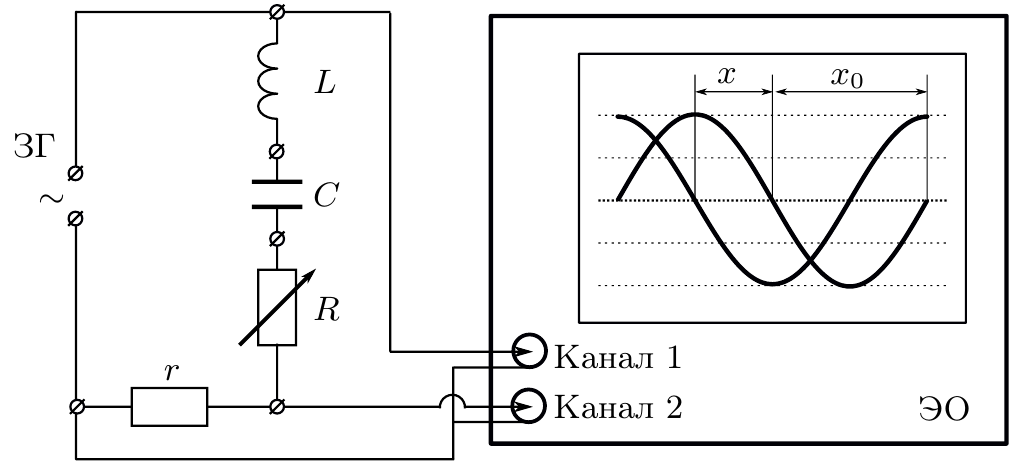
\includegraphics[width=6cm]{res/scheme1.png}
    	\caption{Схема установки для исследования сдвига фаз между током и напряжением}
    	\label{fig:s1}
    \end{figure}
    
    Сигнал, пропорциональный току, снимается с сопротивления $r$, пропорциональный напряжению, -- с генератора. Оба сигнала подаются на осциллограф (ЭО), имеющий два канала вертикального отклонения. Измерение разности фаз можно проводить одним из двух описанных выше способов.
    
    Схема фазовращателя, применяемого в данной работе, изображена на рис. \ref{fig:s2}. Она содержит два одинаковых резистора $R_1$, смонтированных на отдельной плате, магазин сопротивлений $R$ и магазин ёмкостей $C$.
    
    \begin{figure}[h!]
    	\centering
    	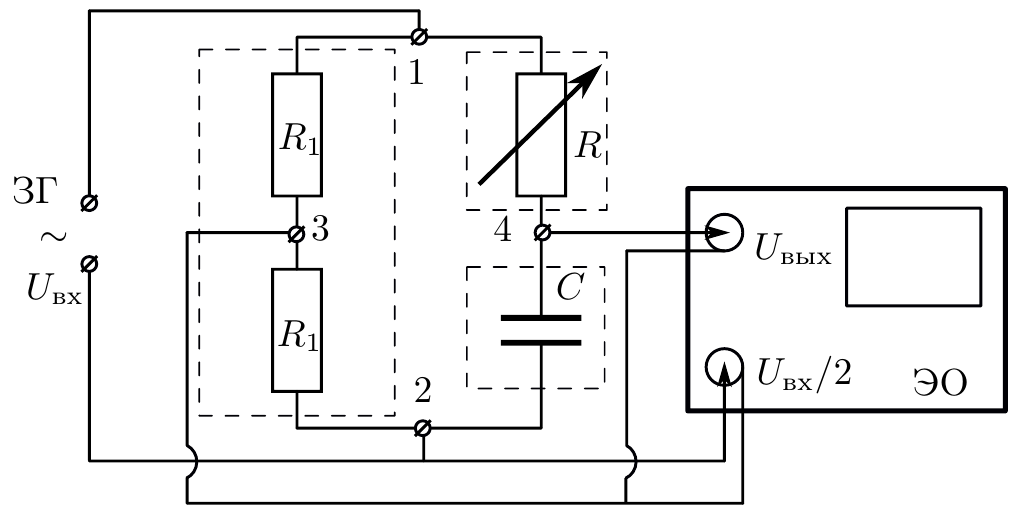
\includegraphics[width=6cm]{res/scheme2.png}
    	\caption{Схема установки для исследования фазовращателя}
    	\label{fig:s2}
    \end{figure}
    
    Сдвигу $\psi = \pi/2$ соответсвует случай, когда на фазовой диаграмме (рис. \ref{fig:ph}) треугольник 124 прямоугольный равнобедренный.
    
    \begin{figure}[h!]
    	\centering
    	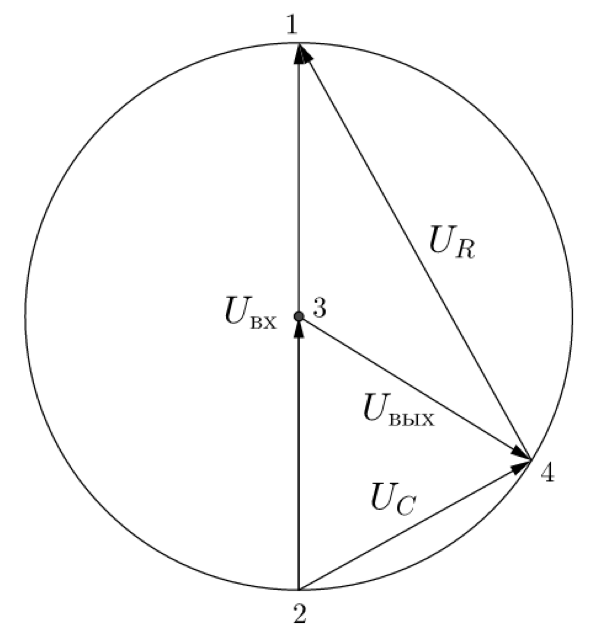
\includegraphics[width=6cm]{res/phase.png}
    	\caption{Фазовая диаграмма}
    	\label{fig:ph}
    \end{figure}
    

\section*{Ход работы}

\subsection*{Исследование сдвига фаз в RC-цепи}

Для начала занесём параметры установки в таблицу \ref{tab:t1}.

\begin{table}[H]
	\caption{Характеристики установки}
	\begin{tabular}{cc}
\toprule
$r$, Ом & $R_L$, Ом \\
\midrule
12.2 & 31.5 \\
\bottomrule
\end{tabular}


	\label{tab:t1}
\end{table}

Установим $C = 0.5$ мкФ, $\nu = 1$ кГц. Тогда реактивное сопротивление $X_1=1/(\omega C)=1/(2\pi C)=318$ кОм.
Будем увеличивать сопротивление R от нуля до $10 X_1$, измеряя сдвиг фаз $\psi$ для каждого значения R.
Все измерения и их обработку занесём в таблицу \ref{tab:tC}. Построим график зависимости $\cot(\psi)=f\left( \omega C R_\Sigma \right)$.

\begin{table}[H]
	\caption{Измерения и их обработка при исследовании сдвига фаз в RC-цепи}
	\begin{tabular}{cccccc}
\toprule
$R$, кОм & $x$, дел & $x_0$, дел & $\psi$, рад & $\cot(\psi)$ & $\omega C R_\Sigma$ \\
\midrule
0    & 8.0 & 17.0 & 1.5 & 0.09 & 0.04 \\
159  & 6.5 & 18.5 & 1.1 & 0.50 & 0.54 \\
318  & 4.5 & 17.5 & 0.8 & 0.96 & 1.04 \\
636  & 3.0 & 20.0 & 0.5 & 1.96 & 2.04 \\
954  & 2.0 & 20.0 & 0.3 & 3.08 & 3.04 \\
1272 & 1.5 & 20.0 & 0.2 & 4.16 & 4.03 \\
1908 & 1.0 & 20.0 & 0.2 & 6.31 & 6.03 \\
\bottomrule
\end{tabular}
	\label{tab:tC}
\end{table}

Как известно, комплексный импеданс RLC-цепочки:
$$ Z = R + j\omega L + 1/(j \omega C)$$
Сдвиг фаз между током и напряжением:
$$\tan \psi = \frac{\omega L - 1/(\omega C)}{R}$$
В нашем случае $L=0$, поэтому в теории
$$\cot \psi = \omega R C.$$

    \begin{figure}[h!]
    	\centering
    	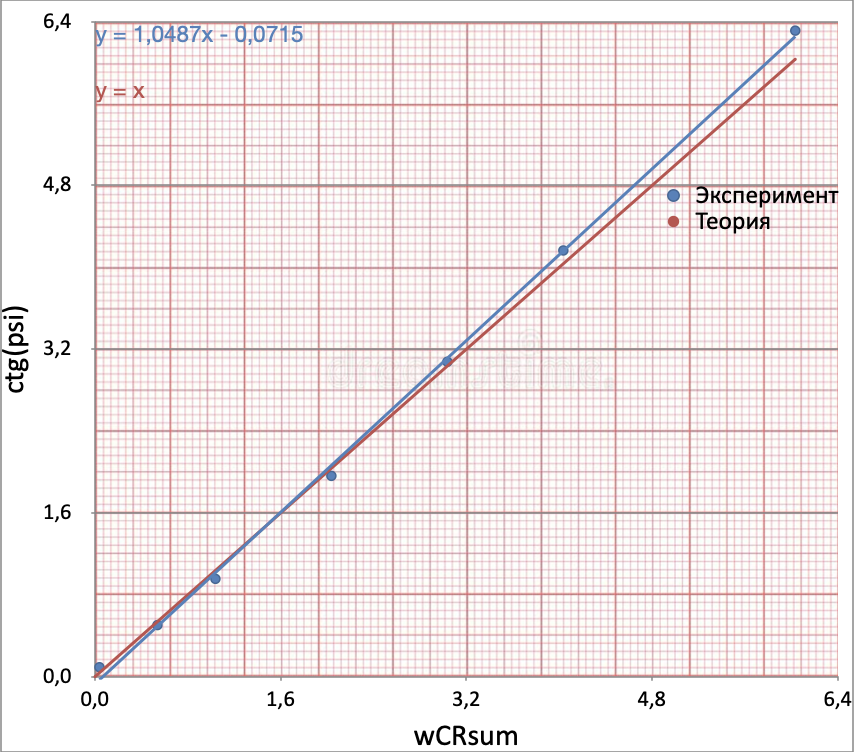
\includegraphics[width=10cm]{src/RC.png}
    	\caption{График экспериментальной и теоретической зависимости $\cot(\psi)=f\left( \omega C R_\Sigma \right)$}
    	\label{fig:plRC}
    \end{figure}

Как видно из графика, теоретическая зависимость отлично сходится с экспериментальной.

\subsection*{Исследование сдвига фаз в RC-цепи}

Установим $L = 50$ мГн, $\nu = 1$ кГц. Аналогично предыдущему пункту, снимем зависимость $\psi(R)$ и занесём все измерения и их обработку в таблицу \ref{tab:tL}. Построим график зависимости $\cot(\psi)=f\left( R_\Sigma/(\omega L) \right)$.

\begin{table}[H]
	\caption{Измерения и их обработка при исследовании сдвига фаз в RL-цепи}
	\begin{tabular}{cc}
\toprule
$R$, Ом & $\sigma_R$, мА \\
\midrule
36.25 & 0.20 \\
35.14 & 0.40 \\
\bottomrule
\end{tabular}

	\label{tab:tL}
\end{table}

    \begin{figure}[h!]
    	\centering
    	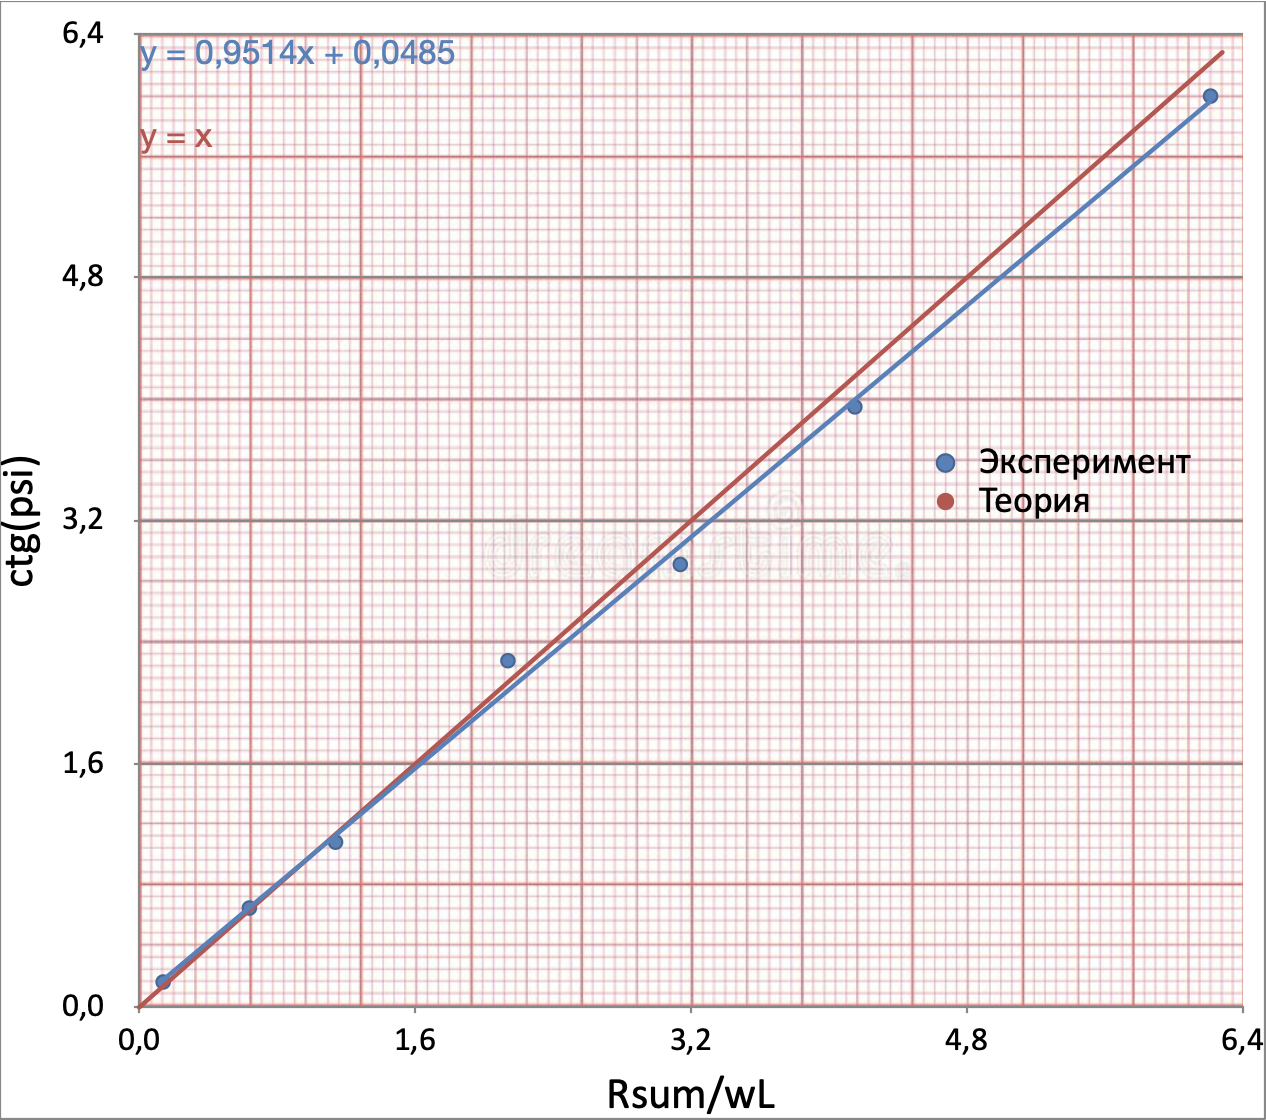
\includegraphics[width=10cm]{src/RL.png}
    	\caption{График экспериментальной и теоретической зависимости $\cot(\psi)=f\left( R_\Sigma/(\omega L) \right)$}
    	\label{fig:plRL}
    \end{figure}
    
    В данном случае $C \rightarrow \infty$. Поэтому теоретически 

    $$\cot \psi = R/(\omega L).$$
    График также хорошо сходится с теоретическим.



\subsection*{Исследование зависимости сдвига фаз от частоты в RLC-цепи}

Установим $L = 50$ мГн, $C = 0.5$ мкФ и $R = 0$ Ом. Резонансная частота $\nu_0 = 1/(2\pi \sqrt{LC}) = 1006.6$ Гц. Будем исследовать резонанс в интервале частот $865 < \nu < 1150$ Гц, т. к. при таких частотах $\|\psi \|<\pi/3$. Снимем зависимомть фазы от частоты. Аналогичные измерения проведём при $R = 100$ Ом. Занесём измерения и их обработку в таблицу \ref{tab:rcl}. Построим график $\|\psi\|=f \left( \nu/\nu_0 \right)$.

\begin{table}[H]
	\caption{Фазово-частотные характеристики в RLC-цепи}
	\begin{tabular}{c|cccc|cccc}
\toprule
$\nu$, Гц & $x_0$, дел & $x$, дел & $\psi$, рад &  $\nu/\nu_0$ 
          & $x_0$, дел & $x$, дел & $\psi$, рад &  $\nu/\nu_0$\\

 & \multicolumn{4}{c}{$R$ = 0 Ом} & \multicolumn{4}{c}{$R$ = 100 Ом} \\

850  & 19.0 & 7.0  & 1.158 & 0.845 & 19.0 & 3.5 & 0.579 & 0.845 \\
900  & 17.5 & 5.5  & 0.987 & 0.894 & 17.5 & 2.5 & 0.449 & 0.894 \\
940  & 17.0 & 4.0  & 0.739 & 0.934 & 16.7 & 1.3 & 0.245 & 0.934 \\
970  & 16.3 & 2.2  & 0.424 & 0.964 & 16.0 & 1.0 & 0.196 & 0.964 \\
990  & 16.0 & 1.2  & 0.236 & 0.984 & 15.7 & 0.5 & 0.100 & 0.984 \\
1000 & 39.0 & 1.1  & 0.089 & 0.994 & 39.0 & 0.1 & 0.008 & 0.994 \\
1010 & 38.0 & 1.0  & 0.083 & 1.004 & 38.0 & 0.0 & 0.000 & 1.004 \\
1030 & 37.0 & 4.0  & 0.340 & 1.023 & 36.0 & 1.5 & 0.131 & 1.023 \\
1060 & 36.5 & 7.0  & 0.603 & 1.053 & 36.0 & 2.5 & 0.218 & 1.053 \\
1100 & 35.0 & 10.0 & 0.898 & 1.093 & 35.0 & 4.0 & 0.359 & 1.093 \\
1150 & 33.5 & 11.0 & 1.032 & 1.143 & 33.0 & 5.5 & 0.524 & 1.143 \\
\bottomrule
\end{tabular}

	\label{tab:rcl}
\end{table}

    \begin{figure}[h!]
    	\centering
    	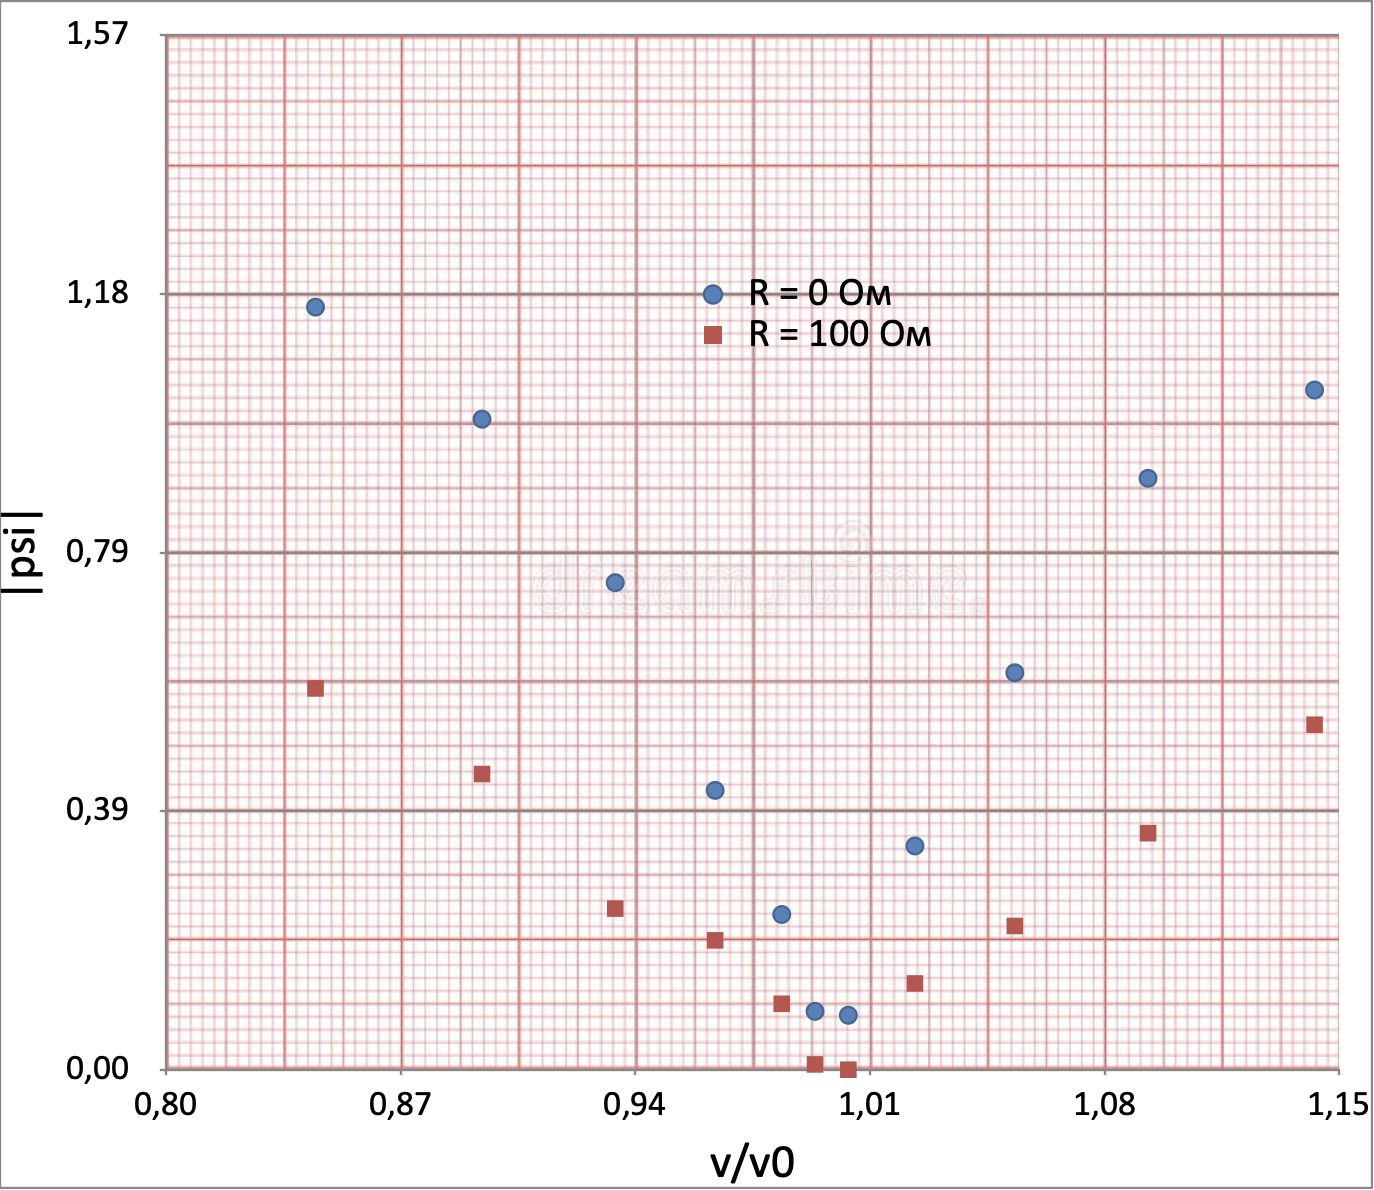
\includegraphics[width=10cm]{src/RLC.png}
    	\caption{Фазово-частотный график для RLC-цепочки}
    	\label{fig:pltrlc}
    \end{figure}
    
Определим добротность из графика: 
$$Q=\nu_0/(2\Delta \nu),$$
где $2\Delta \nu$ -- ширина графика при сдвиге фаз $\psi = \pi/4$. Для случая $R=100$ Ом определить ширину на уровне $\pi/4$ затруднительно. Поэтому определим её на уровне $\pi/8$ и тогда 
$$\tan \pi/8 = \frac{\omega L - 1/(\omega C)}{R} = Q \frac{\left(\frac{\omega}{\omega_0}\right)^2-1 }{\frac{\omega}{\omega_0}} =Q \frac{(1+x)^2-1}{(1+x)^2} \approx Q 2 x_{\psi = \pi/8},$$
откуда легко вычислить добротность.
Также определим добротность по формуле
$$Q=\frac{1}{R}\sqrt{\frac{L}{C}}.$$
Результаты занесём в таблицу \ref{tab:q}. Как видно из таблицы, результаты довольно хорошо согласуются.

\begin{table}[H]
	\caption{Результаты измерений добротности}
	\begin{tabular}{c|c|c}
\toprule
 & $R$ = 0 Ом & $R$ = 100 Ом \\
$Q_\text{теор}$ & 7.2 & 2.2 \\
$Q_\text{граф}$ & 6.8 & 2.1 \\
\bottomrule
\end{tabular}

	\label{tab:q}
\end{table}

\subsection*{Исследование работы фазовращателя}

Соберём схему, изображённую на рисунке \ref{fig:s2}. Установим $C = 0.5$ мкФ и $\nu = 1$ кГц. Подберём сопротивление, при котором сдвиг фаз равен $\pi/2$: R = 1920 Ом. Теоретическое значение $R=1/(\omega C)=2$ кОм. Как видно, значения совпадают в пределах погрешности.

\section*{Вывод}

В ходе работы была изучена зависимость сдвига фаз между током и напряжением от сопротивления в цепи в RC, RL, RLC контурах. Была определена добротность колебательного контура без резистора 100 Ом и с ним, снята зависимость сдвига фаз от частоты вблизи резонанса.
Было определено сопротивление, при котором амплитуды напряжений на резисторе и конденсаторе в фазовращателе совпадают.

\newpage
\begin{thebibliography}{9}
	\bibitem{Siv} Сивухин Д. В. \emph{Общий курс физики. Том 3 Электричество и магнетизм}, 2004
	\bibitem{kirich} Кириченко Н.А. \emph{Электричество и магнетизм.}, 2011
	\bibitem{max} \emph{Лабораторный практикум по общей физике. В 3 томах. Том 2. Электричество и магнетизм: учебное пособие} под ред. А. В. Максимычева, М. Г. Никулина
\end{thebibliography}

\end{document}
